\let\negmedspace\undefined
\let\negthickspace\undefined
\documentclass[journal]{IEEEtran}
\usepackage[a5paper, margin=10mm, onecolumn]{geometry}
%\usepackage{lmodern} % Ensure lmodern is loaded for pdflatex
\usepackage{tfrupee} % Include tfrupee package

\setlength{\headheight}{1cm} % Set the height of the header box
\setlength{\headsep}{0mm}     % Set the distance between the header box and the top of the text

\usepackage{gvv-book}
\usepackage{gvv}
\usepackage{cite}
\usepackage{amsmath,amssymb,amsfonts,amsthm}
\usepackage{algorithmic}
\usepackage{graphicx}
\usepackage{textcomp}
\usepackage{xcolor}
\usepackage{txfonts}
\usepackage{listings}
\usepackage{enumitem}
\usepackage{mathtools}
\usepackage{gensymb}
\usepackage{comment}
\usepackage[breaklinks=true]{hyperref}
\usepackage{tkz-euclide} 
\usepackage{listings}
% \usepackage{gvv}                                        
\def\inputGnumericTable{}                                 
\usepackage[latin1]{inputenc}                                
\usepackage{color}                                            
\usepackage{array}                                            
\usepackage{longtable}                                       
\usepackage{calc}                                             
\usepackage{multirow}                                         
\usepackage{hhline}                                           
\usepackage{ifthen}                                           
\usepackage{lscape}
\usepackage{circuitikz}
\tikzstyle{block} = [rectangle, draw, fill=blue!20, 
    text width=4em, text centered, rounded corners, minimum height=3em]
\tikzstyle{sum} = [draw, fill=blue!10, circle, minimum size=1cm, node distance=1.5cm]
\tikzstyle{input} = [coordinate]
\tikzstyle{output} = [coordinate]


\begin{document}

\bibliographystyle{IEEEtran}
\vspace{3cm}

\title{4.12.45}
\author{AI25BTECH110031 \\ Shivam Sawarkar}
 \maketitle
% \newpage
% \bigskip
{\let\newpage\relax\maketitle}

\renewcommand{\thefigure}{\theenumi}
\renewcommand{\thetable}{\theenumi}
\setlength{\intextsep}{10pt} % Space between text and floats


\numberwithin{equation}{enumi}
\numberwithin{figure}{enumi}
\renewcommand{\thetable}{\theenumi}

\textbf{Question(4.12.45)} Find the equation of the set of points $P$ the sum of whose distances from $A(4, 0, 0)$ and $B(-4, 0, 0)$ is equal to 10. \\ 
\textbf{Solution:} \\ 
We want the locus of points $\vec{p} \in \mathbb{R}^3$ such that
\begin{align}
\norm{\vec{p}-\vec{A}}+\norm{\vec{p}-\vec{B}} = 10,
\end{align}
where
\begin{align}
\vec{A} = \myvec{4 \\ 0 \\ 0}, \quad
\vec{B} = \myvec{-4 \\ 0 \\ 0}.
\end{align}

\textbf{Step 1 - Decomposition of $\vec{p}$:}

Define the unit vector along the foci axis:
\begin{align}
\vec{e} = \frac{\vec{A} - \vec{B}}{\norm{\vec{A}-\vec{B}}}
= \frac{\myvec{8 \\ 0 \\ 0}}{8} = \myvec{1 \\ 0 \\ 0}.
\end{align}

Decompose $\vec{p}$ into parallel and perpendicular components:
\begin{align}
\vec{p} = (\vec{e}^\top \vec{p})\,\vec{e}
+ \big( I - \vec{e}\vec{e}^\top \big) \vec{p}.
\end{align}

Let:
\begin{align}
\alpha := \vec{e}^\top \vec{p}, \quad
R := I - \vec{e}\vec{e}^\top.
\end{align}
Then the perpendicular squared component is:
\begin{align}
s := \|R\vec{p}\|^2.
\end{align}

\textbf{Step 2 - Distances to the foci:}

\begin{align}
\norm{\vec{p}-\vec{A}}
= \sqrt{(\alpha - 4)^2 + s}, \quad
\norm{\vec{p}-\vec{B}}
= \sqrt{(\alpha + 4)^2 + s}.
\end{align}

The condition becomes:
\begin{align}
\sqrt{(\alpha - 4)^2 + s} + \sqrt{(\alpha + 4)^2 + s} = 10.
\end{align}

\textbf{Step 3 - Eliminate square roots:}

Square both sides and rearrange to eliminate the radicals.
After algebraic manipulation, we obtain:
\begin{align}
-36\,\alpha^2 - 100\,s + 900 = 0.
\end{align}

The equation becomes:
\begin{align}
-36\,\vec{p}^\top (\vec{e}\vec{e}^\top) \vec{p}
- 100\,\vec{p}^\top R \vec{p}
+ 900 = 0.
\end{align}

\begin{align}
\vec{p}^\top\left(
-36\,\vec{e}\vec{e}^\top - 100\,R
\right)\vec{p} + 900 = 0.
\end{align}

\textbf{Step 4 - Simplify using $R = I - \vec{e}\vec{e}^\top$:}
\begin{align}
-36\,\vec{e}\vec{e}^\top - 100(I - \vec{e}\vec{e}^\top)
= -100I + 64\,\vec{e}\vec{e}^\top.
\end{align}

Thus:
\begin{align}
\vec{p}^\top\left(
I - \frac{64}{100}\vec{e}\vec{e}^\top
\right)\vec{p} = 9.
\end{align}

\begin{align}
\boxed{
\vec{p}^\top
\myvec{
\tfrac{1}{25} & 0 & 0 \\ 
0 & \tfrac{1}{9} & 0 \\ 
0 & 0 & \tfrac{1}{9}
}
\vec{p} = 1,
}
\end{align}
which is the equation of a prolate spheroid with semi-axes $5,3,3$.

\begin{figure}[H]
    \centering
    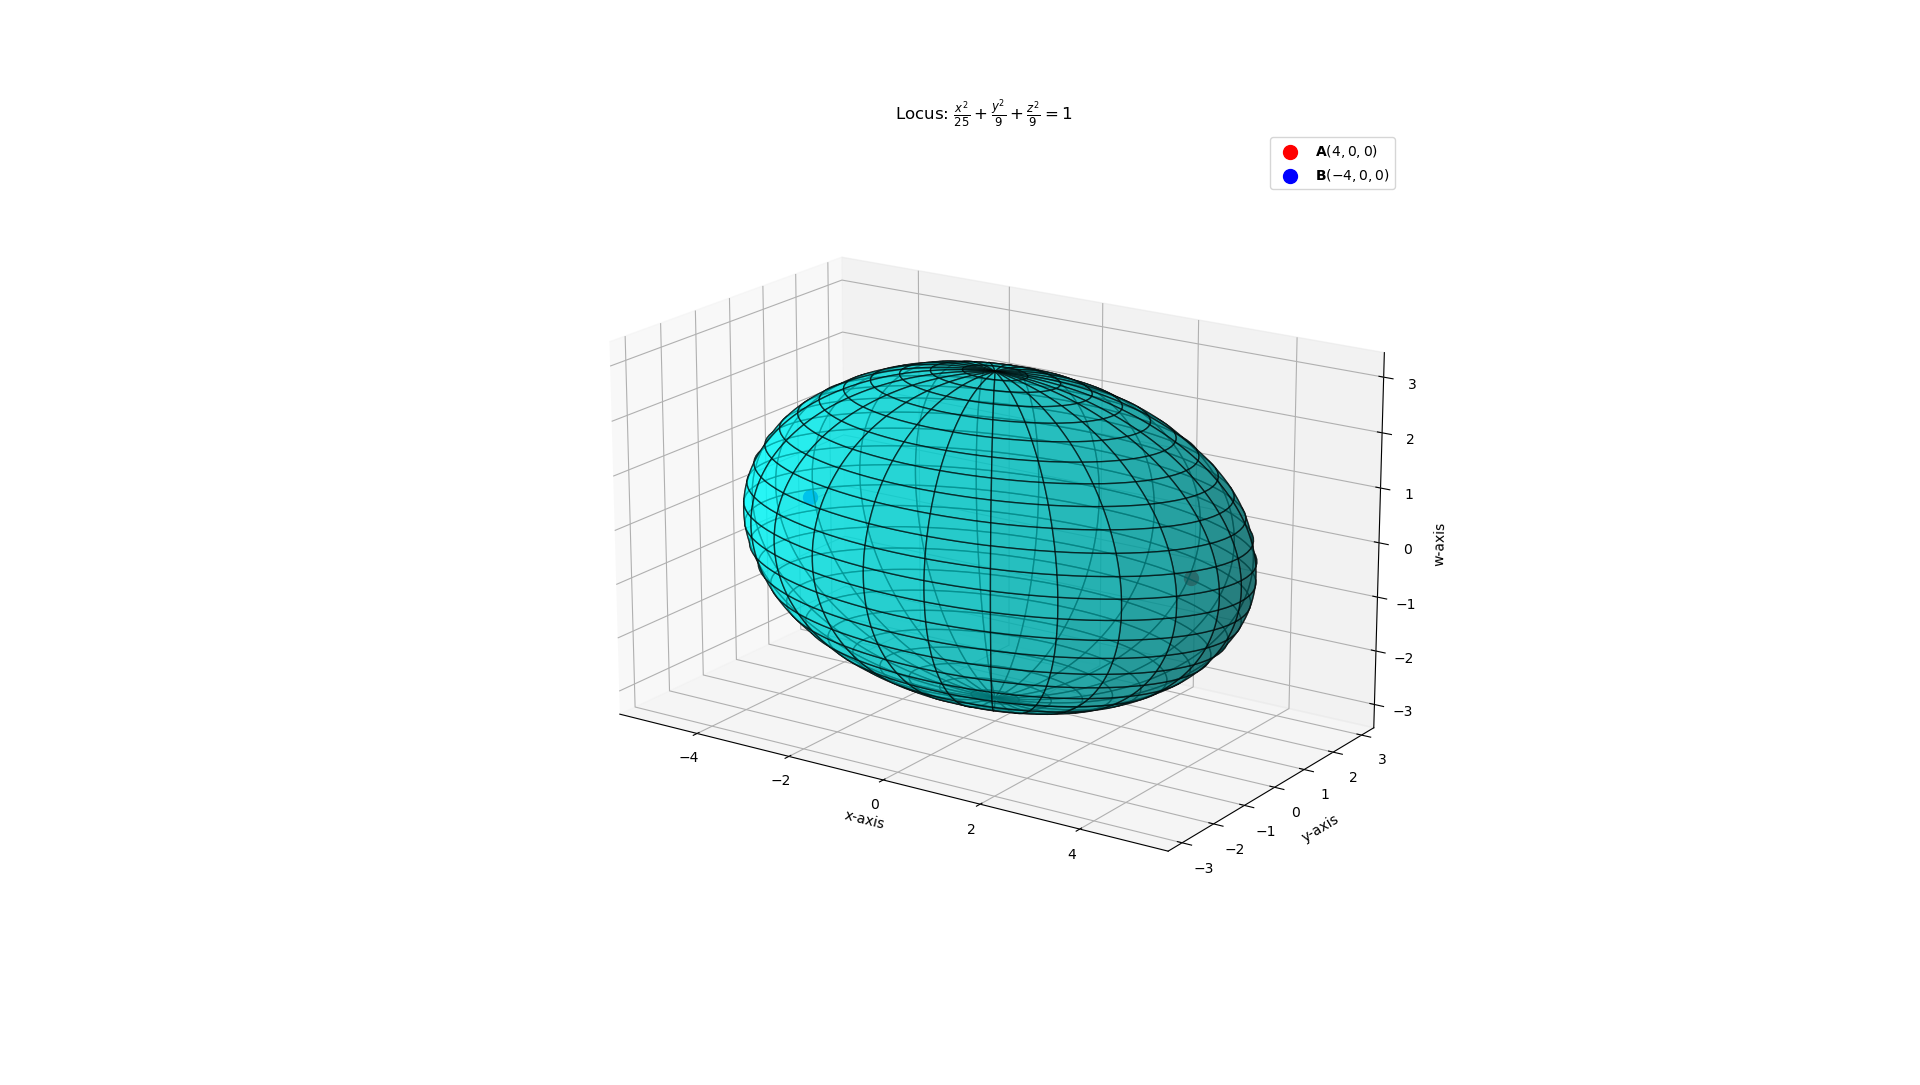
\includegraphics[width=1\linewidth]{figs/plot9.png}
    \caption{}
    \label{fig:placeholder}
\end{figure}





\end{document}